% !TeX root = ../main.tex

\begin{translation}
\label{cha:translation}

\title{外文资料的书面翻译}
% \maketitle

\section{Salto-1P的极限加速度(14 g)重复空间跳跃}
论文索引:
Haldane D W, Yim J K, Fearing R S. Repetitive extreme-acceleration (14-g) spatial jumping with Salto-1P[C]//2017 IEEE/RSJ International Conference on Intelligent Robots and Systems (IROS). IEEE, 2017: 3345-3351.

{\kaishu 摘要——}在这项工作中,我们提出了一种新的机器人系统Salto-1P,用于探索极限跳跃运动。 Salto-1P重0.098kg,有效腿长为14.4cm。 该机器人能够执行1.25m的竖向垂直跳跃,连续跳至1m以上的高度,并水平跳越2m。 Salto-1P使用气动推进器和惯性尾翼来控制其在空中的姿态。 线性化的Raibert步进控制器足以实现不受限制的就地跳跃,并通过外部位置反馈实现向前和向后运动。 我们对极限跳跃运动进行了研究,其中机器人仅在地面上花费其时间的7.7\%,在站立阶段经历的加速度是地球重力的14倍。实验收集到的772个跳跃的数据集用于确定Salto-1P可实现的水平和垂直脉冲范围。
\subsection{引言}
跳跃动物可以通过连续的大型(超过2m)跳跃在林木繁杂的环境中移动,如丛猴。这种机器人运动的跳跃模式非常有趣,因为它可以在复杂的地形中快速移动,并为机器人与环境的交互方式增加了灵活性。机器人跳得越远,它越能将环境离散化,清除较大的间隙和障碍,并使路径规划变得更容易[7]。先前的工作表明,可以连续执行两次高振幅跳跃的机器人能够从墙壁上弹出来获得能量和高度[12]。精通跳跃运动的机器人将能够以以前无法使用的新方式在环境中移动。
极端的跳跃运动的特点是跳跃距离较大(超过1m),而站姿时间短,这带来了一些挑战。为了探索这种运动模式,机器人需要能够跳得较高,反复执行并控制着陆。即使满足了这些条件,极端的跳跃运动仍可能带来未知的挑战和特性。
例如:占空系数定义为在地面上花费的时间与总步幅持续时间的比率,并且经常用于评估步态的动态特征。跑步动物的典型占空系数为0.36-0.5 [10],大多数跑步机器人的占空系数约为0.5。 在这项工作中开发的机器人的占空系数低至0.077,低于以最高速度运行的猎豹单肢的最低观测占空系数[15]。 机器人在站立时经历的加速度反复超过地球重力的14倍。
有许多高性能的腿式机器人,但没有一个专门研究极限跳跃运动。 能够重复跳跃的动力自主跑步机器人[17],[5],[11],[14],[19],[24],[34]尚未展示出跳跃高度超过0.5m的能力( 除了Salto-1P(这项工作)。 这些机器人的跳跃高度与其特征尺寸相当,并且其相对较小的最大跳跃无法实现Campana和Laumond提出的敏捷运动[7]。
\begin{figure}[h]
  \centering
   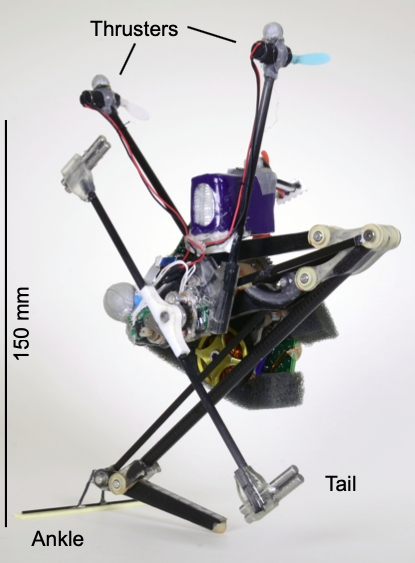
\includegraphics[height=6cm]{fig1.png}
   \caption*{图~1\hskip1em Salto-1P带推进器照片,完全蹲下}
   \label{tab:figure1}
 \end{figure}
跳得最高的机器人会爆炸性地释放预先存储的能量来为自己的跳跃提供动力。这种存储的能量可能是使用字面意义的爆炸进行跳跃的机器人中的化学推进剂,例如Sandia hopper[31]或Boston Dynamics的SandFlea。其他高跳机器人将能量存储在平行弹性的腿部机构中,并使用机械擒纵机构在单个脉冲中将其转换为动能[20],[6],[35],[28],[1], [22],[29],[23],[33],[18],[32]。目前,所有可以跳高1米以上的动力自动机器人(Salto [12]和Salto-1P除外)都使用并行弹性或爆炸驱动策略。这些机器人的问题在于它们无法执行连续运动所需的受控重复跳跃。高跳的平行弹性机器人需要较长的时间才能准备下一次跳跃。这种行为尚未在爆炸式机器人中得到证明,这可能是因为跳跃的肢体太僵硬而无法使站立时间足够长,无法与地面进行有意义的交互。
先前的工作表明,Salto(全称:地形障碍物上的跳跃运动)是一种具有串联弹性执行器和可变机械增益(SE + MA)肢体的机器人(请参见[13],[12],[25] ),可以跳过1米高。 SE + MA的驱动策略使机器人可以在没有较长缠绕时间的情况下达到此高度,并且不会因机械擒纵机构或依靠爆炸性化学推进剂而妨碍腿的可控制性。 Salto的主要缺点是它纯粹是平面的。不能拒绝任何远离其操作平面的干扰,因此机器人只能执行少量跳跃动作而不会跌落。此外,Salto仅具有内部传感,并且缺少能够使其执行扩展的一系列重复跳跃的控制器。
在这项工作中,我们通过创建具有完全姿态控制的Salto-1P改进版,来实现极限跳跃运动。我们实现了简单的Raibert控制器[26],以使Salto-1P能够在水平面上反复跳跃,并探究了单姿态事件可能产生的脉冲范围。
第二节概述了机器人硬件,姿态控制器,运动控制器和实验程序的开发。第三部分给出了姿态控制和跳跃实验的结果,第四部分讨论了结论。


\subsection{实验方法}
\subsubsection{姿态控制}
Salto-1P的第一个挑战是启用姿态控制,以便可以调节腿部的落地接触角。原始的Salto是平面的,并使用了质量平衡的惯性尾巴来控制其在矢状面中的方向[12]。该尾巴为进行跳墙动作所需的激进姿态重新定位提供了动力[12]。对于Salto-1P,我们决定保留平衡的尾巴,以快速进行下垂方向的调整,并以足够的控制量最小地补充它,以使机器人保持直立,并具有正确的偏航角。稳定极端加速度跳跃的挑战是相对于飞行时间而言,站立时间较短。任何仅在站姿(如脚或脚踝关节)中操作的稳定方法都必须在0.05s站姿期间纠正姿势,并将起飞角速度误差降低到足够低的程度,以使机器人位于
在下一个姿势事件(0.5秒后)时,其期望的落地接触角误差只有几度。
单足机器人有许多稳定方法(参见Sayyad等人的评论[27])。出于测试目的,最常见的是将单脚架安装到动臂上,由于机器人的质量轻且垂直偏移量大,因此不适合Salto-1P。另一种选择是将腿安装在机器人身体质心的两个自由度伺服关节上,就像Raibert Hopper [26]和3D Bow Bow Hopper [34]一样。对于Salto-1P,这没有吸引力,因为身体的移动范围受到限制,极大地限制了其可以承受的角度脉冲。任何具有偏移质量的重定位策略(例如二自由度尾翼[8])都会给Salto-1P带来困难,因为其特征是较大的加速姿态会在尾翼执行器上产生较大的扭矩要求。其他单足机器人(例如[16] [30])选择静态稳定的脚,并避免会导致机器人离开其支撑多边形的跳跃。这种方法对于Salto-1P是站不住脚的,它可以水平跳两米。
几个跳跃机器人在跳跃后使用空气动力学表面滑翔[32] [21] [9]。空气动力学表面因其低质量和在空中传播时施加力的能力而引人注目(不只是站姿)。缺点是与地面移动相关的雷诺数需要的尺寸很大,并且它们施加的力取决于速度,因此垂直跳跃的机器人失去了顶点的控制权。我们选择了一种紧凑的气动稳定方法,该方法使用图1所示的推进器,而不依赖于速度。这些推进器是安装在“V”形结构中的商用小型四旋翼(Cheerson CX-10)螺旋桨叶片,带有围绕重心的力矩臂,使控制侧倾角(80mm)优先于偏航角(40mm)。通过在相同方向上驱动两个推进器来产生侧倾扭矩。偏航转矩由差动电动机命令产生。推进器组件成功地稳定了机器人(参见图4和5),净重为0.0044kg。
\subsubsection{机器人硬件}
Salto-1P是Salto机器人的改进版本[​​12]。 Salto的串联弹性执行器和机构的几何形状在Salto-1P中得以保留。但是,一些连杆已经过重塑,以使Salto-1P的蹲伏度低于Salto,从而通过增强连杆的功率调节效果来增加可达到的跳跃高度[13]。还使用拓扑优化对机身进行了重新设计,以创建高质量效率,低柔顺性的结构。观察到Salto的塑料尾部变速箱造成了很多不可靠因素后,该尾部变速箱已升级为Salto-1P铝壳钢制齿轮[12]。
与Salto一样,Salto-1P也由ImageProc 2.5\footnote{Embedded PCB: https://github.com/biomimetics/imageproc.pcb}机械手控制板[2]控制。尾部和推进器马达由板载H桥驱动。 Salto-1P使用定制的BLDC电机驱动器,该驱动器比Salto使用的COTS驱动器更小且质量更轻。 imageProc记录来自电动机驱动器和板载6轴IMU的遥测,频率为1kHz。
Salto-1P用半球形橡胶脚趾(IE7000,创新聚合物)与地面接触。将脚趾材料样品从测试室的地毯样品上摩擦,同时力传感器(nano43,ATI)记录的数据确定了摩擦系数μ= 0.79。该摩擦系数足够高,以确保脚趾在实验过程中不会打滑。当机器人完全蹲下时,它放在脚踝结构上(如图1所示),该结构允许静态稳定的静止位置。脚踝的高度应使重心位于机器人脚趾的后面。
\begin{figure}[h]
  \centering
   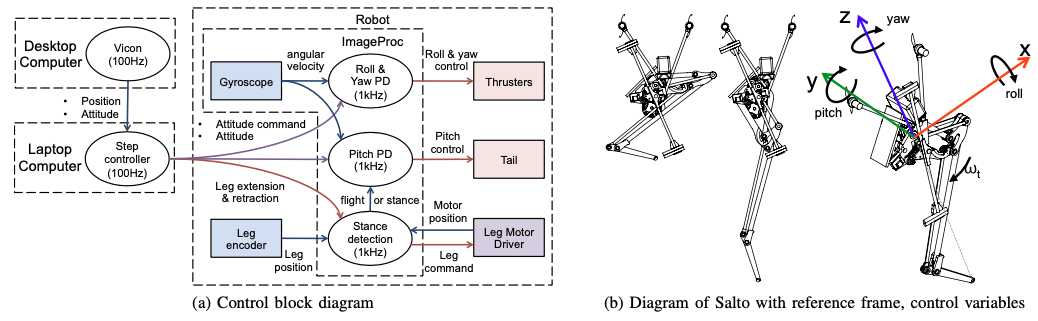
\includegraphics[height=4cm]{fig2.png}
   \caption*{图~2\hskip1em 整体系统框图和Salto-1P参考系}
   \label{tab:figure2}
 \end{figure}

\begin{table}[htb]
  \centering
  \begin{minipage}[t]{0.8\linewidth}
  \caption*{表~1\hskip1em 机器人平台数据}
  \label{tab:table1}
    \begin{tabularx}{\linewidth}{lXX}
      \toprule[1.5pt]
      & {\textbf{Salto}}[12] & {\textbf{Salto-1P}} \\\midrule[1pt]
      质量(kg) & 0.1000 & 0.0981 \\
      有效腿长(m) & 0.138 & 0.144 \\
      最大跳跃高度(m) & 1.007 & 1.252 \\
      垂直跳跃敏捷性(m/s) & 1.75 & 1.83 \\
      \multicolumn{3}{l}{\textit{最大控制力矩(Nm):}} \\
      俯仰 & 0.029 & 0.034 \\
      横滚 & 0 & 0.0078 \\
      偏航 & 0 & 0.0039 \\
      \bottomrule[1.5pt]
    \end{tabularx}
  \end{minipage}
\end{table}
\subsubsection{跳跃控制器}
Salto被设计为运行中弹簧加载的倒立摆(SLIP)模型的实例[4],因此可以使平台的控制尽可能简单。目标是使Salto的动力学模型为加载弹簧的无质量腿上的质点。 Salto的脚尖沿一条直线移动,使腿的质量最小化,腿的运动机制是平衡的,以使连杆的运动不产生身体旋转,惯性尾巴达到质量平衡,并且身体的质量得到集中[13],[25]。这是与Acrobot jumper相反的设计方法,该机器人使用具有非线性控制的最小机械设计,并且在保持平衡的同时几乎不会滑动[3]。 Salto通过这种方式设计,类似于无电缆的0.098千克Raibert hopper[26],而将一个腿部角度定位伺服器替换成了推进器,可以控制偏航角,并且可以跳高1.25m。
为了找到最简单的解决方案,我们选择了基于Raibert步进控制器[26]的线性控制器,用于我们的初始实验。
与Raibert步进控制器一样,控制被分解为三个部分:跳跃高度,尾部速度和水平速度。
弹跳高度是通过在地面上施加固定推力来设置的。 Raibert在[26]中指出,对于每个推力值,此固定推力策略都收敛到唯一的稳态顶点高度。通过选择触地之前的腿缩回长度和机器人接触地面时触发的腿延伸距离(通过监视串联弹性执行器中的弹簧的偏转来检测)来指定推力。
Salto-1P的平衡尾巴类似于Raibert跳跃机的平衡机身。但是,由于尾部无限制地旋转,因此其角度并不重要,我们仅关注其角速度。在站立阶段,驱动尾部电动机的H桥处于制动模式,以降低尾部速度。这对于维持控制权很重要:机尾可产生的控制扭矩会随着机尾速度线性降低。如果没有制动,则尾部将加速至电动机的自由运行速度,并且机器人无法保持对其运动的控制。
水平速度通过在触地时选择合适的腿角来控制。为了简单起见,我们使用偏航-俯仰-俯仰欧拉角来参数化旋转。机器人连接的参考框架如图2b所示。由于Salto-1P的惯性尾部在俯仰轴上的控制权要大于推进器在横滚轴上提供的控制权,因此将操纵引导至矢状面,并且所需的偏航角为0。考虑到所需的重心位置和速度,触地横滚和俯仰角通过以下方式选择:
$$\phi=-k_{P_x}sat(x_d-x,x_{max})-k_{V_x}(\dot{x}_d-\dot{x})$$
$$\theta=k_{P_y}sat(y_d-y,y_{max})+k_{V_y}(\dot{y}_d-\dot{y})$$

其中$\phi$是俯仰角,$\theta$是侧倾角,$sat(u)$是饱和函数,该函数会限制由于位置误差引起的角度指令。$x$是矢状平面中的位置坐标,$y$是水平坐标。
\begin{figure}[h]
  \centering
   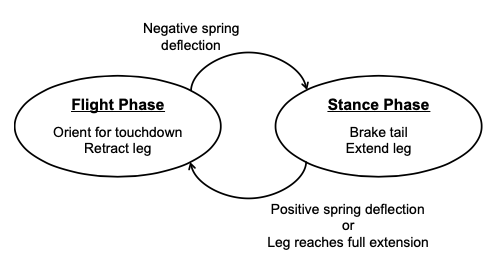
\includegraphics[height=4cm]{fig3.png}
   \caption*{图~3\hskip1em 站立和飞行控制}
   \label{tab:figure3}
 \end{figure}
\subsubsection{实验过程}
为了测试姿态控制执行器的稳定能力,将机器人依次从偏航轴,俯仰轴和横滚轴悬吊下来,并手动施加脉冲干扰。在此实验中,姿态控制器试图保持固定角度;使用外部运动跟踪(Optitrack)观察到了角度扰动和随后的恢复。使用来自车载陀螺仪的数据估算脉冲的大小。
为了提供位置反馈,在Vicon运动捕捉环境中进行了跳跃实验。房间中的可跟踪区域在地面上的尺寸为$2\times3$米。 Vicon的位置和方向测量值以100Hz的频率传递到笔记本电脑上的ROS地面站。地面站通过低通滤波器的离散微分从Vicon位置测量中估算出机器人身体速度。地面站使用上面详述的步进控制器计算了所需的腿长和着陆角,并将这些命令以及Vicon姿态测量值通过XBee无线发送给机器人。发送Vicon测量的姿态以及姿态命令,可防止由于陀螺仪积分误差而导致机载姿态估计值漂移。控制流程如图2a所示。
\subsection{实验结果}
\subsubsection{姿态稳定}
图4显示了Salto-1P在偏航,俯仰和横摇中的5\%恢复时间与微扰脉冲的关系。 Salto-1P从惯性扰动中恢复的速度比侧倾或偏航更快,因为惯性尾翼提供的扭矩大于推进器。注意,0.010kg,0.14m的惯性尾部可以平衡的最大角冲量是有限的。它不能超过$H_t=I\omega$,其中$I$是尾部的惯性,而$\omega$是最大尾部角速度。 Salto-1P上的惯性尾部$H_t=3.5mNm-s$。推力器配置为优先控制横滚其次偏航(请参见表1),其结果如图4所示。机器人从侧倾轴上的干扰脉冲中恢复得比偏航轴更快。
图5显示了跳跃实验过程中姿态控制器的性能。横滚轴和偏航轴(图5(A),(B))的阻尼低于设定值0.1弧度的规则偏差。如图5(C)所示,推进器电动机饱和后,更激进的增益不会产生更好的性能。需要更多的执行机构权限来改善定位。惯性尾翼提供了更多的控制权,触地时的典型俯仰误差小于0.01弧度,如图5(D)所示。尾部电动机(图5(E))在站立阶段制动,以使其减速。起飞后,尾部马达会尽最大努力将机身重新定位到下一个设定点。
\begin{figure}[h]
  \centering
   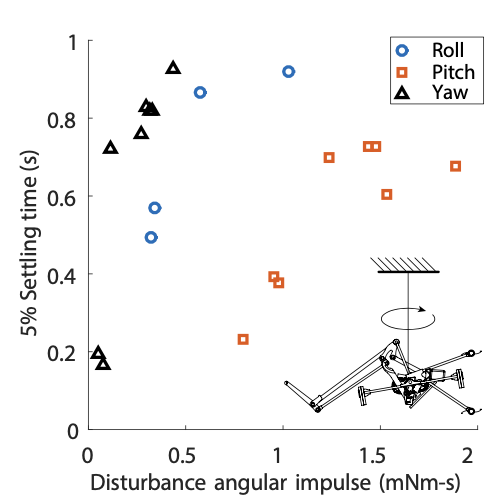
\includegraphics[height=7cm]{fig4.png}
   \caption*{图~4\hskip1em Salto-1P稳定在最大超调量与干扰冲量的5%之间的时间。插图动画显示了用于滚动测试的实验装置。}
   \label{tab:figure4}
 \end{figure}
 \begin{figure}[h]
  \centering
   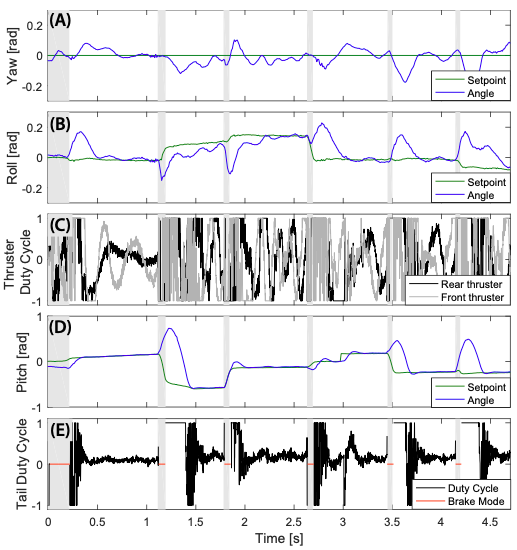
\includegraphics[height=7cm]{fig5.png}
   \caption*{图~5\hskip1em 跳跃实验中的姿态控制器性能。(A)偏航角和设定点 (B)侧倾角和设定点 (C)推进器马达占空比 (D)俯仰角和设定点 (E)尾部马达占空比。 站立阶段以灰色显示。}
   \label{tab:figure5}
 \end{figure}
 \begin{figure}[h]
  \centering
   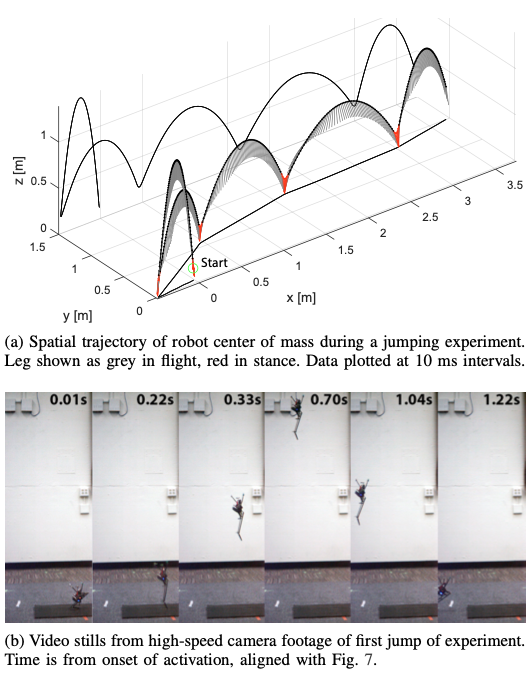
\includegraphics[height=8cm]{fig6.png}
   \caption*{图~6\hskip1em 向前运动测试的示例数据和视频静止图像。}
   \label{tab:figure6}
 \end{figure}
\subsubsection{跳跃运动}
图6a显示了前跳实验中Salto-1P的空间轨迹。来自同一实验的高速视频的静止图像显示在图6b中。机器人开始完全蹲下,脚踝静态稳定,重心位于脚趾后方。 Salto-1P最具活力的跳跃发生在它完全蹲伏的位置时,其中SE+MA跳跃机构最有效[13][12]。因为质心在脚趾后面,所以此初始跳跃是向后的。此初始配置已用于所有跳跃实验,因为第一次跳跃会立即建立极高的跳跃运动所需的高能量状态。向后的方向会扰动运动控制器,因此可以探索大范围的跳跃,并且可以研究收敛性。机器人退出实验测试室的可跟踪范围,实验即结束。
图7(A)显示了与图6a所示相同实验的质心高度随时间变化的情况,站立阶段以灰色显示。初始姿态阶段最长,为0.22s,通过SE+MA[13][12]延长了持续时间,这使机器人可以跳得更高。在较大的初始跳跃之后,该跳跃高度收敛到由该实验的腿推力确定的较小高度。此实验的平均站立时间为0.057s(不包括初始站立时间);平均飞行时间为0.68s,平均占空比为0.077。在此实验中,电动机完成的累积机械功如图7(B)所示。电机在初始姿态阶段输入1.45J的能量,其中1.2J作为质量能量的外在中心,机械效率为83\%。后续跳跃的能量消耗较少。该系列弹性腿能够被动地存储和返还平均65\%的动能;电机每跳输入0.3J即可保持高度,用于克服摩擦和冲击造成的损失。
在观察到的最快持续水平速度为3.6m/s的情况下,机器人的腿部电机每次跳跃消耗15J电能(在站立阶段使用7J),跳跃周期为0.66s。由于空中腿部控制器的行为失调,在飞行中浪费了8J。这对应于该运行的6.6的比电阻。
\begin{figure}[h]
  \centering
   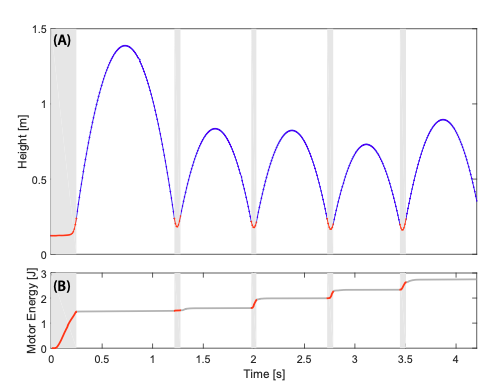
\includegraphics[height=6cm]{fig7.png}
   \caption*{图~7\hskip1em 高度增益和反复跳跃的能量统计。站立时间以灰色显示。(A)质心的高度 (B)从电动机输入的累积机械能。}
   \label{tab:figure7}
 \end{figure}
\subsubsection{运动控制器}
运动控制器的目标是允许Salto-1P重复跳跃,以探索可访问的跳跃行为的范围。我们执行了原地跳跃测试(其中机器人尝试保持固定的x-y位置)和前进后退(其中所需位置向前和向后移动以产生周期运动)。图8a显示了前后运动实验期间Salto-1P质心的位置。在这里,控制器的目的是保持0º偏航角和零横向位移。在该实验中,腿部推力产生的平均跳跃高度为0.65m。在0m处初始停留3秒后,以锯齿状将命令的x位置从0扫到2m。锯齿重复10次,在此期间Salto-1P共进行174次跳跃。除了几个偏差外,横向位置保持在所需横向位置的0.5m以内。机器人在前到后锯齿端点处速度方向改变处过冲。这是由于质心速度误差的激进增益引起的,该误差引起了Salto-1P的动态特性,而不适合此运动任务。 Salto-1P质心加速度的大小如图8b所示。
在原地跳跃中,Salto-1P由于尾部具有出色的俯仰控制,因此可以将脚部放置在横向0.65m和矢状0.3m的区域内。
\begin{figure}[h]
  \centering
   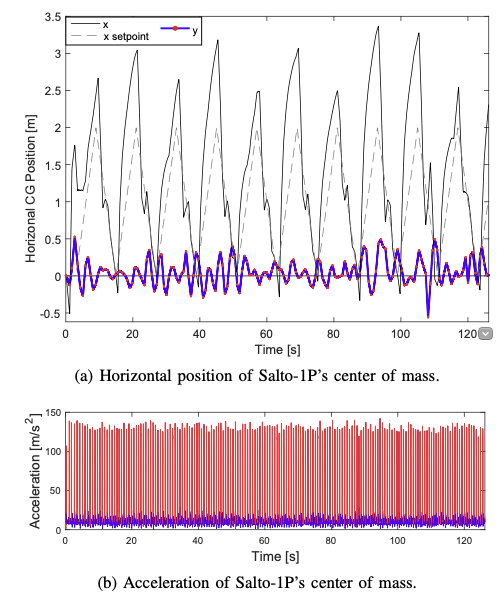
\includegraphics[height=10cm]{fig8.png}
   \caption*{图~8\hskip1em 在向前-向后跳跃实验(总共174次跳跃)过程中,机器人质心的运动。 迹线的红色部分表示站立周期。}
   \label{tab:figure8}
 \end{figure}
\subsubsection{行为探究}
随着机器人的运行,我们试图探索可行的跳跃行为的空间。我们进行了一系列实验,改变了腿的推力命令,并让运动控制器发出了会干扰机器人稳态运动行为的命令。实际上,这意味着要进行向前,向后和原地跳跃实验,并获得一组高度激进的增益,从而产生较大的水平速度。
图9a显示了772个实验观察到的跳跃中的每个的垂直和前后脉冲。大多数数据聚集在原地跳跃实验产生的$\Delta v_x=0$附近。图9b显示了横向与前后脉冲;在前后运行的实验的驱动下,数据聚集在$\Delta v_y=0$附近,并在$\Delta v_x$处有一定分布。通过前向-后向运行试验探索了非零水平脉冲,发现了最大的值和最激进的增益。最大的单个脉冲接近垂直,幅度为$\Delta v=8.94m/s$。机器人无法跳到$\Delta v_z=2m/s$以下。造成困难的原因是,姿态控制执行器在下一个姿势事件之前没有足够的时间来重新定位机器人。这些数据是可达到的跳跃的子集;更好的勘探方案将更彻底地确定Salto-1P跳跃能力的极限。
\begin{figure}[h]
  \centering
   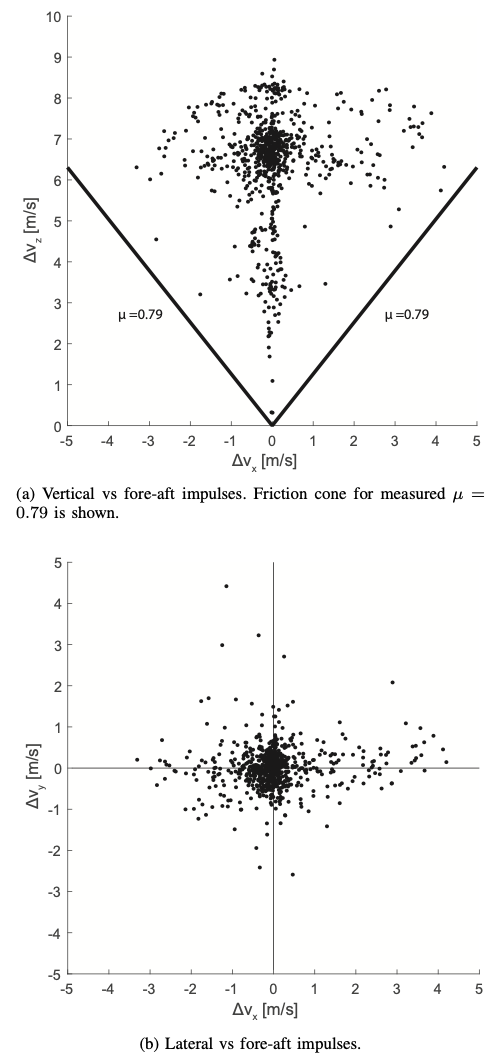
\includegraphics[height=14cm]{fig9.png}
   \caption*{图~9\hskip1em 每个观察到的站立时间的脉冲 (N = 772)}
   \label{tab:figure9}
 \end{figure}

 \subsection{结论与展望}

在这项工作中,我们介绍了先前开发的机器人Salto[12]的改进版本,称为Salto-1P。该机器人比之前的机器人轻2克,可以跳高0.245m,垂直跳动敏捷度为1.83m/s,是所有电池供电机器人的最高记录。为此,我们开发了一种轻量的姿态控制方案,该方案适用于高度灵活的0.1公斤以下单脚机器人。两个气动推进器与惯性尾翼相结合,使机器人可以控制其在空中的姿态。惯性尾部在抵抗扰动方面比推进器更有效,而推进器在跳跃试验中经常被驱使达到饱和。机器人在横滚轴和偏航轴上具有更大的控制权限,将扩大机器人的运行范围。
姿态控制方案使Salto-1P可以在刚性水平面上连续执行多次跳跃(一次试验最多174次)。基于Raibert步进控制器的简单线性化控制器用于机器人的全局位置控制;我们演示了原地跳跃以及向前和向后运行。姿态执行器在飞行阶段而不是在姿态阶段的操作意味着可以使用更小,功能更弱的执行器。推进器可能会作用几百毫秒,而基于地面的解决方案将被限制为≈50毫秒的站立时间。
Salto-1P能够探索极限跳跃运动,证明能够以低至0.077的占空比连续跳越1米高。尽管这种形式的运动带来了挑战,但适当的机器人硬件的选择/构造意味着简单的Raibert控制器能够带动稳定的运动和一系列动态操纵。经过反复的实验,我们能够探索Salto-1P的性能指标,如图9所示。
这项工作表明,Salto-1P具有高度敏捷的运动能力,每姿态最大$\Delta v$为8.9m/s。它具有足够的原始性能,可以作为实验评估最近开发的弹道计划框架的有效平台[7]。然而,仍然缺乏对平台的完全控制,特别是急停的着陆控制和精确的落脚点控制。未来的工作将针对落脚点控制器的开发。
\newline

{\heiti 参考文献} \newline
[1] R. Armour, K. Paskins, A. Bowyer, J. Vincent, W. Megill, and R. Bomphrey, “Jumping robots: a biomimetic solution to locomotion across rough terrain,” Bioinspir. Biomim., vol. 2, no. 3, pp. S65–82, 2007. \newline
[2] S. S. Baek, F. L. Garcia Bermudez, and R. S. Fearing, “Flight control for target seeking by 13 gram ornithopter,” IEEE Int. Conf. Intell. Robot. Syst., pp. 2674–2681, 2011. \newline
[3] M. D. Berkemeier and R. S. Fearing, “Tracking fast inverted trajecto- ries of the underactuated acrobot,” IEEE Trans. Robot., vol. 15, no. 4, pp. 740–750, 1999. \newline
[4] R. Blickhan, “The spring-mass model for running and hopping,” J. Biomech., vol. 22, no. 11-12, pp. 1217–1227, 1989. \newline
[5] A. Brill, A. De, A. Johnson, and D. Koditschek, “Tail-assisted rigid and compliant legged leaping,” IEEE Int. Conf. Intell. Robot. Syst., pp. 6304–6311, 2015. \newline
[6] J. Burdick and P. Fiorini, “Minimalist jumping robots for celestial exploration,” Int. J. Rob. Res., vol. 22, no. 7-8, pp. 653–674, 2003. \newline
[7] M. Campana and J.-P. Laumond, “Ballistic motion planning,” in IEEE Int. Conf. Intell. Robot. Syst., 2016, pp. 1410–1416. \newline
[8] E. Chang-Siu, T. Libby, M. Brown, R. J. Full, and M. Tomizuka, “A nonlinear feedback controller for aerial self-righting by a tailed robot,” in IEEE Int. Conf. Intell. Robot. Syst., 2013, pp. 32–39. \newline
[9] A.L.Desbiens,M.Pope,F.Berg,Z.E.Teoh,J.Lee,andM.Cutkosky, “Efficient jumpgliding: Theory and design considerations,” IEEE Int. Conf. Robot. Autom., pp. 4451–4458, 2013. \newline
[10] C. T. Farley, J. Glasheen, and T. A. McMahon, “Running springs: speed and animal size.” Jnl. Exp. Biol., vol. 185, pp. 71–86, 1993. \newline
[11] C. Gehring, S. Coros, M. Hutter, and R. Siegwart, “An optimization approach to controlling jump maneuvers for a quadrupedal robot,” Dyn. Walk., 2015. \newline
[12] D. W. Haldane, M. M. Plecnik, J. K. Yim, and R. S. Fearing, “Robotic vertical jumping agility via series-elastic power modulation,” Sci. Robot., vol. 1, no. 1, 2016. \newline
[13] D. W. Haldane, M. Plecnik, J. K. Yim, and R. S. Fearing, “A power modulating leg mechanism for monopedal hopping,” IEEE Int. Conf. Intell. Robot. Syst., pp. 4757–4764, 2016. \newline
[14] G. C. Haynes, J. Pusey, R. Knopf, A. M. Johnson, and D. E. Koditschek, “Laboratory on legs: an architecture for adjustable morphology with legged robots,” University of Pennsylvania, Philadelphia, PA, Tech. Rep., 2012. \newline
[15] P. E. Hudson, S. a. Corr, and A. M. Wilson, “High speed galloping in the cheetah (Acinonyx jubatus) and the racing greyhound (Canis familiaris): spatio-temporal and kinetic characteristics.” J. Exp. Biol., vol. 215, no. 14, pp. 2425–34, 2012. \newline
[16] F. Iida, R. Dravid, and C. Paul, “Design and control of a pendulum driven hopping robot,” in IEEE Int. Conf. Intell. Robot. Syst., 2002, pp. 2141–2146. \newline
[17] A. M. Johnson and D. E. Koditschek, “Toward a vocabulary of legged leaping,” IEEE Int. Conf. Robot. Autom., pp. 2568–2575, 2013. \newline
[18] G.-P.Jung,C.S.Casarez,S.-P.Jung,R.S.Fearing,andK.-J.Cho,“An integrated jumping-crawling robot using height-adjustable jumping module,” IEEE Int. Conf. Robot. Autom., pp. 4680–4685, 2016. \newline
[19] G. Kenneally, A. De, and D. E. Koditschek, “Design principles for a family of direct-drive legged robots,” IEEE Robot. Autom. Lett., vol. 1, no. 2, pp. 900–907, 2016. \newline
[20] M. Kovac, M. Fuchs, A. Guignard, J.-C. Zufferey, and D. Floreano, “A miniature 7g jumping robot,” in IEEE Int. Conf. Robot. Autom., 2008, pp. 373–378. \newline
[21] M. Kovacˇ, Wassim-Hraiz, O. Fauria, J. C. Zufferey, and D. Floreano, “The EPFL jumpglider: A hybrid jumping and gliding robot with rigid or folding wings,” IEEE Int. Conf. Robot. Biomimetics, pp. 1503–1508, 2011. \newline
[22] F. Li, W. Liu, X. Fu, G. Bonsignori, U. Scarfogliero, C. Stefanini, and P. Dario, “Jumping like an insect: Design and dynamic optimization of a jumping mini robot based on bio-mimetic inspiration,” Mechatronics, vol. 22, no. 2, pp. 167–176, 2012. \newline
[23] M. Noh, S.-W. Kim, S. An, J.-S. Koh, and K.-J. Cho, “Flea-Inspired Catapult Mechanism for Miniature Jumping Robots,” IEEE Trans. Robot., vol. 28, no. 5, pp. 1007–1018, 2012. \newline
[24] H. W. Park, S. Park, and S. Kim, “Variable-speed quadrupedal bound- ing using impulse planning: Untethered high-speed 3D Running of MIT Cheetah 2,” in IEEE Int. Conf. Robot. Autom., vol. 2015-June, no. June, 2015, pp. 5163–5170. \newline
[25] M. M. Plecnik, D. W. Haldane, J. K. Yim, and R. S. Fearing, “Design exploration and kinematic tuning of a power modulating jumping monopod,” J. Mech. Robot., vol. 9, pp. 1–13, 2016. \newline
[26] M. H. Raibert, H. B. Brown, and M. Chepponis, “Experiments in balance with a 3D one-legged hopping machine,” Int. J. Rob. Res., vol. 3, no. 2, pp. 75–92, 1984. \newline
[27] A. Sayyad, B. Seth, and P. Seshu, “Single-legged hopping robotics research - A review,” Robotica, vol. 25, no. 05, pp. 587–613, 2007. \newline
[28] S. A. Stoeter, P. E. Rybski, M. Gini, and N. Papanikolopoulos, “Autonomous stair-hopping with scout robots,” IEEE Int. Conf. Intell. Robot. Syst., vol. 1, pp. 721–726, 2002. \newline
[29] T. Tsuda, H. Mochiyama, and H. Fujimoto, “Quick stair-climbing using snap-through buckling of closed elastica,” Int. Symp. Micro- NanoMechatronics Hum. Sci., pp. 368–373, 2012. \newline
[30] T. Wei, G. Nelson, and R. Quinn, “Design of a 5-cm monopod hopping robot,” IEEE Int. Conf. Robot. Autom., pp. 2828–2833, 2000. \newline
[31] B. P. Weiss, “Hop Hopbots!” Sci. News, vol. 159, 2001. \newline
[32] M. A. Woodward and M. Sitti, “MultiMo-Bat: A biologically inspired integrated jumping-gliding robot,” Int. J. Rob. Res., vol. 33, pp. 1511–1529, 2014. \newline
[33] V. Zaitsev, O. Gvirsman, U. Ben Hanan, A. Weiss, A. Ayali, and G. Kosa, “Locust-inspired miniature jumping robot,” in IEEE Int.
Conf. Intell. Robot. Syst., 2015, pp. 553–558. \newline
[34] G. Zeglin and H. B. Brown, “First Hops of the 3D Bow Leg Hopper,” 5th Int. Conf. Climbing Walk. Robot., pp. 357–364, 2002. \newline
[35] J. Zhao, N. Xi, B. Gao, M. W. Mutka, and L. Xiao, “Development of a controllable and continuous jumping robot,” IEEE Int. Conf. Robot. Autom., pp. 4614–4619, 2011. \newline

\end{translation}
